\PassOptionsToPackage{table}{xcolor}
\documentclass[manuscript,nonacm]{acmart}
\AtBeginDocument{%
  \providecommand\BibTeX{{%
    Bib\TeX}}}

\usepackage{amsmath}
\let\Bbbk\relax
\usepackage{amssymb}
\let\Bbbk\relax
\usepackage{pifont}
\usepackage{wasysym}
\usepackage{marvosym}
\usepackage{threeparttable}
\usepackage{textgreek}
\usepackage{paralist}
\usepackage{filecontents}
\usepackage{booktabs}
\usepackage{multirow}
\usepackage{tikz,siunitx}
\usetikzlibrary{shapes.geometric,shapes.symbols}
\usepackage{threeparttable}
\usepackage{enumerate}
\usepackage{comment}

% Commands for Surveyed Works Table
\newcommand{\cmark}{\ding{51}}%
\newcommand{\xmark}{\ding{55}}%
\newcommand{\markA}{\ding{66}}%
\newcommand{\markB}{\ding{71}}%
\newcommand{\markC}{\ding{75}}%
\newcommand{\markD}{\ding{168}}%
\newcommand{\markE}{\ding{169}}%
\newcommand{\markF}{\ding{170}}%
\newcommand{\markG}{\ding{171}}%
\newcommand{\markH}{\ding{92}}%
\newcommand{\markI}{\ding{214}}%
\newcommand{\markJ}{\ding{166}}%
\newcommand{\markX}{\Sagittarius} % heh
\newcommand{\markY}{\Virgo}
\newcommand{\markZ}{\Moon}
\newcommand{\markEtc}{\textbf{?}}
\def\rot{\rotatebox}
\newcommand*\circled[1]{\tikz[baseline=-3pt]{
            \node (X) [shape=circle,scale=0.5,fill=black,text=white,font=\bfseries, text centered, draw,inner sep=0pt] {\strut #1};}}
            
\newcommand{\wc}[1]{\textit{\textcolor{magenta}{#1}}} % Word-Choice macro
\newcommand{\maxnote}[1]{\textit{\textcolor{violet}{#1 --Max}}}
\newcolumntype{P}[1]{>{\centering\arraybackslash}p{#1}}

\begin{document}

\title{PLACEHOLDER}
\author{Max Gao}
% \authornote{Both authors contributed equally to this research.}
\affiliation{%
  \institution{CAIDA/UC San Diego}
  \city{San Diego}
  \state{CA}
  \country{USA}
}
\email{magao@ucsd.edu}

\begin{abstract}
For decades, analysis of network telescope traffic has consistently provided insights into Internet-wide phenomena, \textit{e.g.,} malicious scanning, backscatter from denial-of-service (DoS) attacks, and Internet outages, that impact the security and availability of the Internet.
To better operationalize darknets for their monitoring capabilities, researchers have proposed numerous methodologies that each aim to automate the detection of such events by employing a variety of techniques and leveraging different features of darknet traffic.
Yet despite an abundance of available methodologies, less attention has been directed towards comprehensive assessment of their comparative capabilities due to the availability of labeled datasets, replicability of methodologies, and a unified approach to method validation.
In this report, we survey existing works that propose and evaluate detection such methodologies, \dots

% Analysis of network telescope, or darknet, traffic has provided substantial visibility into the security and availability of the Internet for decades.
% To operationalize darknet monitoring capabilities, researchers have proposed numerous frameworks that automate the detection of Internet-wide events.
% Despite an abundance of available frameworks, less attention has been directed towards systematic comparison of their capabilities. 
% As a result, \dots
% In this report, we survey existing work that proposes and evaluates such frameworks on real-world darknet traffic.
% We review tasks that motivate the techniques each framework employs as well as experimental details of their evaluation; and finally, discuss future \dots
% To more effectively operationalize network telescopes for monitoring the security and availability of the Internet, researchers have proposed a diverse body of frameworks which codify empirical post-hoc analysis techniques.
% Yet, \dots
\end{abstract}

\maketitle

\section{Introduction}

Network telescopes, or darknets, have been instrumental to both researchers and practitioners for their ability to observe Internet-wide phenomena in the unsolicited traffic they receive. 
Over the past two decades, research efforts have shifted from characterizing darknet phenomena and their observable signals towards translating such empirical insights into operationalizable methodologies for monitoring the Internet's security and availability in near real-time.
% This has resulted in a number of methodologies that each leverage different approaches to achieve a common goal of broadly automating darknet event detection. 
% \maxnote{see other papers for enumerating on specific details in intro} As security risks mount along growing volumes of darknet traffic, such methodologies represents a crucial and necessary transition from conventional post-hoc manual traffic analysis workflows. 
% However, the utility of these methodologies depend critically on their accuracy and validity which remain elusive to evaluate due to several challenges that we identify through our survey. 
These efforts have resulted in a variety of methodologies that share the common goal of broadly automating event detection while differing widely in the algorithmic techniques they employ (e.g., statistical forecasting, matrix decompositions, and graph-based models), 
the traffic features they exploit (e.g., packet counts, port sequences, temporal bursts), 
and their operational definition of what constitutes an event (ranging from short-lived scans to sustained probing campaigns).
As security risks mount along growing volumes of darknet traffic, such methodologies represent a crucial and necessary transition from post-hoc manual traffic analysis towards a more \maxnote{dots} means of detection.
However, the utility of these frameworks depend critically on their accuracy and validity, which remain elusive to evaluate due challenges posed by \dots.

% However, as we identify in our suvey, methodologies differ widely in several ways: the algorithmic techniques they employ (e.g., statistical forecasting, matrix decompositions, and graph-based models), the traffic features they exploit (e.g., packet counts, port sequences, temporal bursts), 
% and their operational definition of what constitutes an event (ranging from short-lived scans to sustained probing campaigns).

% Network telescopes, or darknets, have been instrumental to both researchers and practitioners due to their capacity to observe Internet-wide phenomena in the unsolicited traffic they receive. 
% The visibility afforded by these observatories have enabled significant progress in the areas of cybersecurity and censorship, evident in a rich body of work that centers around the study of malicious scanning, denial-of-service attacks, and Internet outages. 
% The visibility afforded by these observatories have enabled significant progress in the areas of cybersecurity and censorship, evident in a rich body of work centered around 
% malicious scanning, denial-of-service events, and Internet outages. 

% Over the past two decades, research efforts have shifted from characterizing darknet phenomena and their observable signals towards translating such empirical insights into operationalizable frameworks for monitoring the Internet's security and availability in near real-time.  
% This has led to the development of a number of frameworks that each share the common goal of automating the detection of events in darknet traffic while taking notably different approaches to doing so\maxnote{feedback: elaborate on the specifics here.}.
% As security risks mount along with growing volumes of darknet traffic, such frameworks represent a crucial and necessary transition from conventional post-hoc manual traffic analysis workflows.
% However, the utility of these frameworks, particularly those more recent that leverage machine learning techniques, depend critically on their accuracy and validity which remain elusive to evaluate due to challenges posed by the diversity of framework detection objectives and approaches.

% As a result, a number of frameworks that each share a common goal of automating event detection within darknet traffic have been proposed.
% This has resulted in a number of proposed frameworks that share a common goal of automating the detection of events within darknet traffic.
% \begin{enumerate}
%   \item Overview of topic - 2 sentences.
%   \item 
%   \item Summary of contributions - 3 sentences.
% \end{enumerate}

% Network telescopes, or darknets, have been instrumental to both researchers and practitioners due to their capacity to observe Internet-wide phenomena in the unsolicited traffic they receive.
% Over the past two decades, research efforts have shifted from characterizing such phenomena and their observable signals towards translating these empirical insights into operationalizable frameworks for monitoring the Internet's security and availability in near real-time.

% Network telescopes, or darknets, have been instrumental to both researchers and practitioners due to their capacity to observe Internet-wide phenomena in the unsolicited traffic they receive.
% Over the past two decades, research efforts have shifted from characterizing such phenomena and their observable signals towards translating empirical insights into operationalizable frameworks for monitoring the Internet's security and availability in near real-time.
% As a result, a large variety of frameworks have been proposed. 
% Each share the same general goal of automating event detection.
% They vary widely in their choice of techniques and selection of darknet traffic features as they are designed with different event definitions in mind.
% \textit{discuss why it's difficult to speculate on their performance without further empirical evaluation.}

% Despite the variety of available frameworks for darknet traffic analysis, selecting the most suitable framework off-the-shelf for a given darknet is challenging.
% While the variety of frameworks is frank

% Traffic Growth
% Complexity Growth - new 

In this report, we survey an extensive body of literature to construct a taxonomy of darknet event detection methodologies followed by a separate taxonomy that details their assessments in empirical evaluations. 
We begin with an overview of prior work that characterizes network telescope traffic and chronicles its major changes in Section~\ref{sec:bg}.
We then describe our taxonomy of methodologies in Section~\ref{sec:frameworks}, comparing\dots\maxnote{brief summary}, followed by a review of their evaluation in Section~\ref{sec:evaluations}.
Finally, using our survey's findings, we conclude with a discussion of challenges in this area as well as directions for future work in Section~\ref{sec:fw}.

% We begin this report with an overview of network telescopes, the traffic they collect, and the types of Internet-wide events inferrable through analysis of such traffic.
% We then survey various frameworks that have been proposed to automate event detection and construct a taxonomy that compares their 1) analysis goals and designs; and 2) performance as informed by empirical evaluations on real-world darknet traffic.
% Using this taxonomy, we identify challenges and opportunities for future research where efforts may yield improvements over the current state-of-art.

\label{sec:bg}
\section{Background}

In this section, we provide a brief overview of network telescopes and findings from prior works that characterize the nature of darknet traffic.

\label{sec:bg:nt}
\subsection{Network Telescopes}

% Brief overview of darknets and their traffic (IBR)
Network telescopes, or darknets, consist of IPv4 address space that receive, but do not respond to, unsolicited Internet traffic via routes announced through the Border Gateway Protocol (BGP).
For decades, researchers have studied this unidirectional traffic to understand its mixtures and origins, attributing its causes to Internet-wide activity ranging from 
malicious scanning~\cite{@@}, residual backscatter from DoS attacks~\cite{@@}, Internet outages~\cite{2011dainotti,2013benson,2015benson,2012dainotti,2021padmanabhan}, and non-trivial network misconfigurations~\cite{@@}.

\begin{enumerate}
    \item three types of Internet-wide activity (summarize findings from each of the past major works, characterization of IBR and its changes, major events studied)
\end{enumerate}

Studies of darknet traffic in 2003 by Yegneswaran et al.~\cite{2004yegneswaran} quantified the volume of traffic and distributions of senders responsible for originating malicious scans 
and estimated that 25 billion Internet-wide scans originate per day.
Pang et al.~\cite{2004pang}\dots
Casado et al.~\cite{2005casado}

% Characterization citations
~\cite{2004yegneswaran,2004pang}

% Outage
~\cite{2011dainotti,2013benson,2015benson,2012dainotti}~\cite{2021padmanabhan}

% Discuss IBR, how it's been analyzed, practical use-cases for security / outage detection

\label{sec:frameworks}
\section{Darknet Event Detection Methodologies}

% In this section, we broadly survey existing methodologies that have been proposed to detect various types of darknet events and discuss their commonalities 
% while emphasizing their differences that pose a challenge to conducting systematic evaluations. \maxnote{revise the takeaway...}
% % In this section, we provide a broad survey of existing frameworks that represent a wide spectrum of techniques proposed to detection various kinds of darknet events.
% We structure our survey by categorizing detection methodologies primarily based on the \textit{type of event} (\textit{e.g.,} scanning, backscatter, and outages) 
% they aim to detect. Within these categories, we review and emphasize two important aspects for each individual framework: 1) the \textit{classes of general techniques} that encompass their employed algorithms; 
% and 2) the \textit{event schema} or unit of detection defined by their authors. 
% Here, we briefly discuss these aspects we consider before expounding on individual works.

% In this section, we broadly survey existing methodologies that have been proposed for detecting various types of darknet activities.
In this section, we provide a broad survey of existing methodologies that have been proposed for detecting darknet activities and 
organize prior works into a taxonomy that identifies the need for a systematic evaluation approach to account for the diversity of methods.
We structure our survey by categorizing detection methodologies primarily based on the type of darknet activity they aim to detect. 
Within these categories, we review and emphasize two important aspects of each methodology: 
1) the class(es) of general \textit{techniques} they employ for detection; and 
2) their definition(s) of an \textit{event} belonging under their broader type of targeted activity.
We briefly discuss these aspects before discussing the methodologies that comprise our taxonomy as shown in Figure~\ref{fig:taxonomy}.


\vspace{0.25em}
\noindent{\textbf{Activity Type(s)}} correspond to existing categories of observed activities in darknet traffic as described in Section~\ref{sec:bg:nt}. 
For each study, we identify these type(s) based on explicitly stated goals of each methodology and empirical results from their evaluation. 
Some methods such as~\ref{@@} are capable of detecting multiple types of activities depending on whether their input traffic is filtered.

% A common case where a single framework can detect multiple types of events 
% While some frameworks can capture multiple types of events, in practice 
% While in practice these are dependent on traffic inputs, we determine detectable activities for each framework based on explicitly stated design goals and evaluation results.

\vspace{0.25em}
\noindent{\textbf{Event Definitions}} refers to attributes represented in the outputs of a given framework.
These attributes derive from packet header fields and implicitly define an instance of a broader type of event.
For example, a framework may define a scanning event using a source-based schema that consists of a timestamp, source IP address, an assigned cluster, and a cluster flag indicating potential malicious intent.

\vspace{0.25em}
\noindent{\textbf{Technique(s)}} differentiate functionalities that specific \textbf{algorithm(s)} undertake within the scope of each methodology.
We identified 7 classes of techniques across our surveyed work which include \textit{dimensionality reduction}, \textit{clustering}, \textit{forecasting}, \textit{thresholding}, \textit{representation learning},
\textit{frequent pattern mining}, and \textit{fingerprinting}. 
To achieve detection objectives, methodologies frequently combine techniques, \textit{e.g.}, reducing the dimensionality of inputs prior to clustering or 
thresholding as a final-pass, semi-automatic means of filtering outputs before manual validation takes place.
% differentiate general functions frameworks leverage, often in combination, to
% achieve their detection objectives. We define 7 classes of techniques which include \textit{dimensionality reduction}, \textit{clustering}, \textit{forecasting}, \textit{thresholding}, \textit{representation learning},
% encompass the specific algorithms employed by each framework and 
% \textit{frequent pattern mining}, and \textit{fingerprinting}.

% \vspace{0.25em}
% \noindent{\textbf{Algorithm(s)}} consist of specific 

% In this section, we provide a broad survey of existing darknet event detection frameworks that exemplify a wide spectrum of 
% different analytical tasks and techniques; in addition, we review the empirical evaluations of these frameworks to consider 
% their efficacy in practice.
% We structure our survey by categorizing proposed frameworks primarily based on the \textit{type of event} (\textit{e.g.}, \textit{scanning}, 
% \textit{backscatter}, and \textit{outages}) they are designed to detect.
% Within these categories, we review and emphasize two important aspects of each individual framework:
% 1) the \textit{classes of general techniques} that encompass their employed algorithms; and
% 2) the \textit{event schema} or unit of detection.
% We define 7 classes of techniques that differentiate the functions of algorithms within the scope of each framework: 
% \textit{dimensionality reduction}, \textit{clustering}, \textit{forecasting}, \textit{thresholding}, \textit{representation learning},
% \textit{frequent pattern mining}, and \textit{fingerprinting}.
% Some frameworks by design are capable of detecting multiple types of events using a combination of different techniques.

% We structure our survey of proposed frameworks by grouping 
% by categorizing frameworks into groups based primarily 
% 1) the primary type of darknet event they were designed to detect; and 
% 2) their definition of 

\begin{figure}
    \begin{tikzpicture}
        \draw (0, 0) node[inner sep=0] {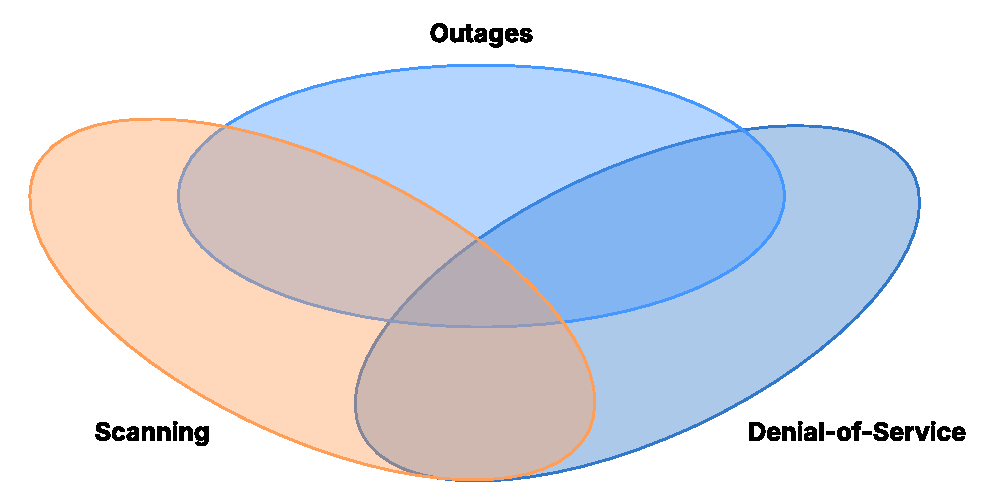
\includegraphics[]{figures/taxonomy.pdf}};
        \draw (-4, -4) node {Kallitsis et al.~\cite{2022kallitsis}};
    \end{tikzpicture}
    \caption{A taxonomy of our \maxnote{number} surveyed works and their methodologies categorized under the broad type of darknet activity they target and specific event definitions.}
    \label{fig:taxonomy}
\end{figure}

\subsection{Scan Detection Methodologies}

Frameworks designed to detect scanning in darknet traffic typically base their event schemas around either source or destination attributes.
Source-based schemas discern various sender behaviors within incoming traffic to a darknet; in contrast, destination-based schemas emphasize specific targets that incoming traffic directs towards.
\vspace{0.25em}

% Frameworks designed to detect scanning events in darknet traffic typically base their event schema on either source or destination attributes.
% Source-based event schemas enable discernment of different types of sender behavior within incoming traffic to a darknet whereas in contrast, 
% destination-based event schemas identify specific targets that incoming traffic is directed towards.


% Enummerate works here
\noindent{\textbf{Sourced-based detection}} occurs at a variety of resolutions, ranging from individual and subnetted addresses to the level of autonomous-systems (ASes).
Several of these leverage representation learning combined with clustering at the level of individual source IPs. \maxnote{revise}
Gioacchini et al.~\cite{@@} propose a domain-specific adaptation of Word2Vec that detect anomalous clusters of senders from their arrival order in packet sequences. 
Kallitsis et al.~\cite{@@} used a more comprehensive set of features to train autoencoders, clustering senders in lower-dimensional embedding space.
Both operate at the level of individual source IP addresses. 

Other closely-related frameworks employ dimensionality reduction techniques that rely on linear methods\footnote{while dimensionality reduction can be considered representation learning, we distinguish the two primarily by linearity of the method}.
In a series of works, Han et al.~\cite{@@} separately apply Non-negative Matrix Factorization and Graphical LASSO alongside ad-hoc thresholding techniques to identify coordinated senders.
Kanehara et al.~\cite{@@} apply 


% Sourced-based Frameworks
% Clustering is a commonly employed technique used to {...}.
% When combined with thresholding, frameworks can to some degree automatically identify clusters worthy of assessment.
% Several works combine representation learning techniques to {...}.

% Han et al. [32, 34 , 35 ] and Kanera
% et al. [ 40 ] applied Non-negative Tucker Decomposition (NTD), Non-negative Matrix Factorization
% (NMF), and Graphical LASSO (GLASSO) to darknet traffic time series before thresholding ouputs
% to identify timeframes of potential coordinated scanning.

% On the other hand, destination-based frameworks focus exclusively on detecting target destionation ports.
% Evrard
% Lagraa
% Ban 

\vspace{0.25em}
\noindent{\textbf{Destination-based detection}}


\subsection{Backscatter Detection Methodologies}


\subsection{Outage Detection Methodologies}


% We review individual components of each framework, considering their impact on \textit{the high-level }
% In addition, we include 
% In this section, we provide a broad survey of existing darknet event detection frameworks that we consider in this report.
% In addition to frameworks themselves, we consider characteristics of their empirical evaluation.

% Table~\ref{tab:frameworks} lists publications we collected, grouped by their authors; groups that consist of multiple works 
% indicate works by similar authors that share significant overlap in their framework design, e.g., proof-of-concepts paired with their mature versions.
% \dots

% \noindent{\textbf{Activity Type(s)}} refer to one or multiple types of events, (\textit{e.g.}, \textit{scanning}, \textit{backscatter}, \textit{outages}, or \textit{misconfigurations}) that a framework is capable of capturing.
% While in practice these are dependent on traffic inputs, we determine detectable activities for each framework based on explicitly stated design goals and evaluation results.

% \noindent{\textbf{Technique(s)}} encompass the specific algorithms employed by each framework and differentiate general functions frameworks leverage, often in combination, to
% achieve their detection objectives. We define 7 classes of techniques which include \textit{dimensionality reduction}, \textit{clustering}, \textit{forecasting}, \textit{thresholding}, \textit{representation learning},
% \textit{frequent pattern mining}, and \textit{fingerprinting}.

% \textbf{Algorithm(s)} 

% \begin{center}
    \begin{table}[]
        \small
        % \scriptsize
        \caption{Characteristics of event detection frameworks proposed in our surveyed literature.}
        \label{tab:frameworks}
        \begin{tabular}{lllclc}
            \toprule
            \multicolumn{1}{c}{Work} & \multicolumn{5}{c}{Framework} \\
            \midrule
            & \rot{45}{i. Activity} & \rot{45}{ii. Technique(s)} & \rot{45}{iii. Algorithm(s)} & \rot{45}{\begin{tabular}[c]{@{}l@{}}iv. Traffic\\ Rep.\end{tabular}} & \rot{45}{\begin{tabular}[c]{@{}l@{}}v. Output\\ Attributes\end{tabular}} \\
            \midrule
            Evrard et al.~\cite{2019evrard}                        & \markX                    & \markB        & Dijkstra's~\cite{1959dijkstra}, K-NN~\cite{1967cover,1989fix} & \markD & Dst. Port \\
            Lagraa et al.~\cite{2017lagraa,2019lagraa}             & \markX                    & \markB        & Louvain~\cite{2006newman,2008blondel} & \markD & Dst. Port \\
            Kallitsis et al.~\cite{2022kallitsis}                  & \markX\markY              & \markI\markA\markB  & Autoencoder Dimensionality Reduction~\cite{2006hinton}, K-Means~\cite{1967macqueen} & \markE & Src. IP   \\
            Iglesias et al.~\cite{2019iglesias}                    & \markX\markY              & \markB\markH  & K-Medoids~\cite{2009park}, Fuzzy-Gustafson~\cite{1999krishnapuram}, MAD-Thresholding~\cite{2004liu} & \markE & Src. IP   \\
            Nishikaze et al.~\cite{2015nishikaze}                  & \markX                    & \markB        & Hierarchical Clustering           & \markE & Src. /16  \\
            Soro et al.~\cite{2020soro}                            & \markX                    & \markB        & Louvain Algorithm~\cite{2006newman,2008blondel} & \markF & Src. AS   \\
            % Cohen et al.~\cite{2020cohen}                          & \markX          & \markA\markB  & Word2vec, DBSCAN & \markF & Dst. Port \\
            Gioacchini et al.~\cite{2021gioacchini,2023gioacchini} & \markX                    & \markA\markB  & Word2Vec~\cite{2013mikolov}, K-Means~\cite{1967macqueen}, K-NN~\cite{1967cover,1989fix}, Louvain~\cite{2006newman,2008blondel} & \markF & Src. IP   \\
            % Gioacchini et al.~\cite{2021gioacchini,2023gioacchini} & \markX                    & \markA\markB  & Word2Vec~\cite{2013mikolov}, K-Means~\cite{1967macqueen}, Louvain ~\cite{2006newman,2008blondel} & \markF & Src. IP   \\
            Han et al.~\cite{2021han,2022han}                      & \markX                    & \markA        & NMF~\cite{2000lee}    & \markG & Src. /16, Dst. Port \\
            Han et al.~\cite{2020han,2022han}                      & \markX\markEtc            & \markA        & GLASSO~\cite{2008friedman} & \markG & Src. /16  \\
            Kanehara et al.~\cite{2019kanehara,2022han}            & \markX                    & \markA\markH  & LRA-NTD~\cite{2015zhou}, FTSD~\cite{2010caiafa}, Otsu-Thresholding~\cite{1979otsu}          & \markG & Src. /16, Dst. Port \\
            Kartsioukas et al.~\cite{2023kartsioukas}              & \markX                    & \markA\markH  & Incremental PCA~\cite{2012arora} & \markG & \textit{TODO} \\
            Ban et al.~\cite{2016ban}                              & \markX                    & \markA        & Frequent Pattern Mining~\cite{2000han,2007han}, Hierarchical Clustering~\cite{2012murtagh}  & \markF\markG & Dst. Port \\ 
            Torabi et al.~\cite{2020torabi,2018torabi}             & \markX                    & \markJ        & Association Rule Mining~\cite{1993agrawal}, DBSCAN~\cite{1996ester} & \markD,\markE & \textit{TODO} \\
            Tanaka et al.~\cite{2023tanaka,2021tanaka}             & \markX                    & \textit{TODO} & \textit{TODO} & Source \\
            Niranjana et al.~\cite{2019niranjana}                  & \markX                    & \markA\markB  & PCA~\cite{1901pearson,1993hotelling} &  Source \\
            Cabana et al.~\cite{2019cabana}                        & \markX                    & \markB\markH  & Conduction Detection Algorithm~\cite{2015lu}, Fastcluster~\cite{2013mullner} & \markD\markE & \textit{TODO} \\
            Shaikh et al.~\cite{2018shaikh}                        & \markX\markY\markZ\markEtc & \textit{TODO} & AdaBoost~\cite{@@}, Gradient Boosting~\cite{@@}, Random Forest~\cite{@@}     & \markE       & \textit{TODO} \\  
            % Ban et al.~\cite{2017ban}                              & \markX          & \markH        & CUMSUM & \markG & \\
            % Bou-Harb et al.~\cite{bouharb2013dfa,2014bouharb}      &  & & & & \\
            % & & & & 
            %  & Src.\& Dst. IP, Src.\&Dest Port,\\
            % \rowcolor{gray!50}
            %  \multirow{-2}{*}{Bou-Harb et al.~\cite{2019bouharb,2015bouharb}}    & \multirow{-2}{*}{\markX\markEtc}  & \multirow{-2}{*}{\markC\markB}  & &  \multirow{-2}{*}{\markE}& Protocol, TTL, Flags\\
            %  \rowcolor{white}
            Zakroum et al.~\cite{2022zakroum,2018zakroum}          & \markX          & \markC\markB  & Spectral Clustering~\cite{2001ng}, LSTM~\cite{1997hochreiter}       & \markG        & Dst. Port \\
            \bottomrule
            \multicolumn{6}{l}{Activities: \markX-Scanning, \markY-DDoS, \markZ-Outage, \markEtc-Misconfiguration} \\
            \rowcolor{white}
            \multicolumn{6}{l}{Techniques:\markA-Dimensionality Reduction, \markB-Clustering, \markC-Forecasting, \markH-Thresholding, \markI-Representation Learning, \markJ-Frequent Pattern Mining, \markH-Fingerprinting} \\
            \multicolumn{6}{l}{Traffic representation: \markD-Graph, \markE-Feature Vector, \markF-Sequences, \markG-Time Series}
        \end{tabular}
    \end{table}
% \end{center}

\label{sec:evaluations}
\section{Empirical Evaluations of Detection Methodologies}

Here, as a complement to the previous section, we provide a concise overview of empirical evaluations conducted on detection methodologies. 
% Since assessing in-practice performance of any given methodology rests on the results of well-designed, experimental evaluation, 

% The utility of event detection frameworks depend on their performance as demonstrated in well-designed, experimental evaluations. 
% We provide a concise overview of the components of such evaluation found in our surveyed literature by assessing their replicability, 
% characteristics of their datasets, and the coverage of side-by-side framework comparisons.

\noindent{\textbf{Limited method replicability.}} 
Less than a third of studies publish source code of their methodologies and of those that do, their releases are seldom packaged as reusable libraries, distributed through package managers, or maintained beyond initial publication. 
While the primary goal of these studies is to disseminate research ideas rather than deliver production-grade software, their codebases nonetheless lack interfaces and clear documentation needed for straightforward implementation and thereby discourages frictionless replication.
% Less than a third of the studies publish accompanying source code of their framework implementation and of those that do, 
% we find that their releases are seldom packaged as reusable libraries, distributed through package managers, or maintained beyond initial publication.
% This aligns with expectations as the primary goal is to disseminate research ideas rather than deliver production-grade software.
% Nonetheless, the condition of the codebases we find often lack interfaces and clear documentation needed for straightforward implementation.

Slightly more than half of the works do, however, provide specifications of the computing environment, \textit{e.g., processor capabilities and memory capacity}, used to run evaluations.
\maxnote{add to significance}

\noindent{\textbf{Non-overlapping datasets.}}
We find little overlap 
Framework evaluations use darknet traffic sourced from a variety of telescopes over different timeframes.
Traffic volumes differ by multiple orders of magnitude and likely in other metrics as well.
\maxnote{table revision: move annotation}

\begin{enumerate}
	\item different datasets are used to evaluate frameworks
	\item These datasets share different characteristics, evident in their traffic volumes and ostensibly other traffic metrics too since they're sourced from different darknets
	\item Also annotations. 
	\item Which annotations are commonly used as ground truth? Mira. Which works?
	\item Epistemic-soundness is an issue, what's used as approximate ground truth? How valid are these annotations?
	\item When ground-truth isn't available, how is performance evaluated?
\end{enumerate}

\noindent{\textbf{Side-by-side methodology comparisons.}}
Slightly fewer than half of our surveyed works evaluate their proposed methodology against a baseline methodology using the same dataset.
Of those, use of a dataset does not extend beyond an individual work, i.e., real-world traffic datasets are not widely shared for researchers to evaluate their methodologies.


\begin{enumerate}
	\item we can't reasonably compare frameworks by their performance on different datasets.
	\item Few works compare different frameworks on the same dataset
	\item What's the highest number of frameworks that use the same dataset?
\end{enumerate}

\begin{table*}[h!]
    \small
    % \centering
    \setlength{\tabcolsep}{4pt}
    \caption{Details of empirical evaluation and traffic datasets found in our surveyed work. Appx. Table~\ref{@@} summarizes referenced telescopes.}
	% \caption{Implementation and evaluation details of our surveyed work. Darknet owner indicates which telescope provided each dataset. Traffic volume is split into packets and bytes.}
    \label{tab:eval}
    \begin{tabular}{@{}lccccccccc@{}}
        \toprule
        & \multicolumn{1}{c}{\textbf{Compari-}} 
        & \multicolumn{2}{c}{\bf Replicability} 
        & \multicolumn{1}{c}{\textbf{Telescope(s)}} 
        & \multicolumn{4}{c}{\bf Dataset Attributes} 
        & \multicolumn{1}{c}{\textbf{Annot-}} \\
        \cmidrule(lr){3-4} \cmidrule(lr){6-9}
        \textbf{Work} & \textbf{son} & \textbf{Code} & \textbf{Specs} &  & \textbf{Duration} & \textbf{Year} & \textbf{Packets} & \textbf{Bytes} & \textbf{ations} \\
        \midrule
        Evrard et al.~\cite{2019evrard}
        &  
        &  & 
        & T3, T6
        & 9m & 2015
        & ${\approx}8\times10^{8}$ & ---
        & Manual \\

        Lagraa et al.~\cite{2017lagraa,2019lagraa}
        &  
        &  & \cmark
        & T6
        & 2y & 2014
        & $2\times10^{9}$ & 500 GB
        & Manual \\

        Soro et al.~\cite{2020soro}
        &  
        &  & 
        & T4
        & 3w & 2019
        & --- & ---
        & Manual \\

        Nishikaze et al.~\cite{2015nishikaze}
        &  
        &  & 
        & T3
        & 28d & 2014
        & $3.03\times10^{8}$ & ---
        &  Manual \\

        Kallitsis et al.~\cite{2022kallitsis}
        & \cite{2021gioacchini}
        & \cmark & \cmark
        & T2
        & 28d & 2016
        & $49\times10^{9}$ & ---
        & Manual, Labeled \\

        Iglesias et al.~\cite{2019iglesias}
        &  
        &  & \cmark
        & T1
        & 1m & 2012
        & --- & 2.1 TB
        &  Manual \\

        Gioacchini et al.~\cite{2021gioacchini,2023gioacchini}
        & \cite{2020cohen}
        & \cmark & \cmark
        & T4
        & 30d & 2021
        & $6.3\times10^{7}$ & ---
        & Labeled \\

        Cohen et al.~\cite{2020cohen}
        & \cite{2016ban}
        &  & \cmark
        & Ad hoc ($\approx$/22)
        & 1y & 2019
        & --- & $3+\,\mathrm{TB}$
        & \wc{manual} \\

        Han et al.~\cite{2021han,2022han}
        & \cite{2020han,2006takeuchi,2019kanehara}
        & \cmark & 
        & T3
        & 1m & 2018
        & --- & ---
        & \wc{manual} \\

        Han et al.~\cite{2020han,2022han}
        & \cite{2006takeuchi}
        & \cmark & \cmark
        & T3
        & 1m & 2018
        & --- & ---
        & \wc{manual} \\

        Kanehara et al.~\cite{2019kanehara,2022han}
        & 
        &  & \cmark
        & T3
        & 6m & 2018
        & --- &
        & \wc{manual} \\

        Ban et al.~\cite{2017ban}
        & \cite{2012ban}
        &  & 
        & T3
        & --- & ---
        & --- & ---
        & Manual \\

        Ban et al.~\cite{2016ban}
        & 
        &  & 
        & T3
        & 1y & 2015
        & $3\times10^{7}$ & ---
        & Manual \\

        Bou-Harb et al.~\cite{2014bouharb}
        &  
        &  & 
        & T7
        & 1m & 2013
        & --- & ---
        &  \\

        Bou-Harb et al.~\cite{2019bouharb,2015bouharb}
        & \cmark
        &  & \cmark
        & T7
        & 1m & 2016
        & --- & 240 GB
        & \wc{manual} \\

        Zakroum et al.~\cite{2022zakroum,2018zakroum}
        & ~\cite{2018zakroum}
        & & \cmark
        & T3, T6
        & 3.5y & 2017
        & $10^{10}$ & $1.5+\mathrm{TB}$
        &  \\

        Zakroum et al.~\cite{2023zakroum}
        & ~\cite{2023zakroum}
        & &
        & T3, T6
        & 4.5y & 2018
        & --- & ---
        & TODO \\

        \midrule
        \textbf{Aggregate}
        & 7/16
        & 4/16 & 7/16
        & 8-24
        & 1w--3.5y & 2012--2021
        & --- & ---
        & --- \\
        \bottomrule
    \end{tabular}
\end{table*}

\label{sec:fw}
\section{Open Challenges and Future Work}

Our survey identifies that while research efforts have been highly productive in generating compelling frameworks for automating darknet event detection, 
critical gaps remain that hinder a comprehensive understanding of their in-practice detection capabilities.

\noindent{\textbf{Curated datasets.}}

Labels applied to a dataset do not necessarily have to be ground truth, e.g., they can be the outputs of other methodologies, but their definitions 
need to be known. 

\begin{enumerate}
	\item Labels
\end{enumerate}

\noindent{\textbf{Systematic evaluation.}}

Although some individual works from our survey evaluate their methodologies with the same metrics, \textit{e.g.,} TP, FP, \dots, 
the

\begin{enumerate}
	\item Discuss need for standardized evaluation metrics
	\item Discuss need for experimental consistency
	\item These depend on reusability of framework implementations
\end{enumerate}

\section{Acknowledgments}
asadfadsf

\section{Appendices}

\begin{table}[httb]
	\small
	\caption{Summary of network telescopes.}\label{tab:telescopes}
	\begin{tabular}{cccc}
		\toprule
		Telescopes & Country & Size & Data availability\\
		\midrule
		\textbf{T1.} UCSD-NT~\cite{caida2025ucsdnt} & US & /9+/10 & Raw traces and flow data \\
		\textbf{T2.} Merit ORION~\cite{orion} & US & $\sim$7 $\times$/16s & Raw trace\\
		\textbf{T3.} NICTER~\cite{nicter2025nt} & JP &  /17, /18, 2$\times$/20 & TCP SYN only, anonymized flow data\\
		\textbf{T4.} Politecnico di Torino \cite{2020soro} & IT & 3 $\times$ /24 & Unknown\\
		\textbf{T5.} Darknet-BR \cite{CunhaCamargo2025darknetbr} & BR & /19 & Unknown\\
		\textbf{T6.} LHS Nancy~\cite{inria2025nt} & FR & /20 & Raw trace\\
		\textbf{T7.} Farsight~\cite{@@} & US & /13 & Private\\
		\bottomrule
	\end{tabular}
\end{table}

\begin{acks}
To Robert, for the bagels and explaining CMYK and color spaces.
\end{acks}

\bibliographystyle{plain}
\bibliography{bib/refs.bib}

\appendix
\section{Research Methods}

\subsection{Part One}

Lorem ipsum dolor sit amet, consectetur adipiscing elit. Morbi
malesuada, quam in pulvinar varius, metus nunc fermentum urna, id
sollicitudin purus odio sit amet enim. Aliquam ullamcorper eu ipsum
vel mollis. Curabitur quis dictum nisl. Phasellus vel semper risus, et
lacinia dolor. Integer ultricies commodo sem nec semper.

\end{document}
\endinput